\chapter{Measurements}
\label{chap:measurements}
For determining the directivity of the smartphone microphone, measurements must be conducted.
This process of determining the measurement set-up is discussed in this chapter. 
The hardware which was at our disposal will be adressed first, because it influenced some choices made.
After that, the application of two different sampling schemes will be discussed, from which one is chosen, and the choice of impulse response technique is discussed.
This chapter is concluded with the measurement set-up, some preliminary results and a recap of this chapter.
A summary of this chapter and an overview of our final measurement set-up (for replication) can be found in Appendix \ref{app:setupoverview}. 

During the measurements there were some drawbacks, which will be explained further in the last section of this chapter (Section \ref{sec:prelim_res}).
A solution will be presented in Chapter \ref{chap:equalization}.
These drawbacks were caused by the response of the acoustic system of the measurement set-up, which had more influence on the results than expected.

\section{Measurement hardware}
% refereren naar appendix hier
\begin{figure}[b!]
        \centering
        \begin{subfigure}[t]{0.4\textwidth}
                \centering
    			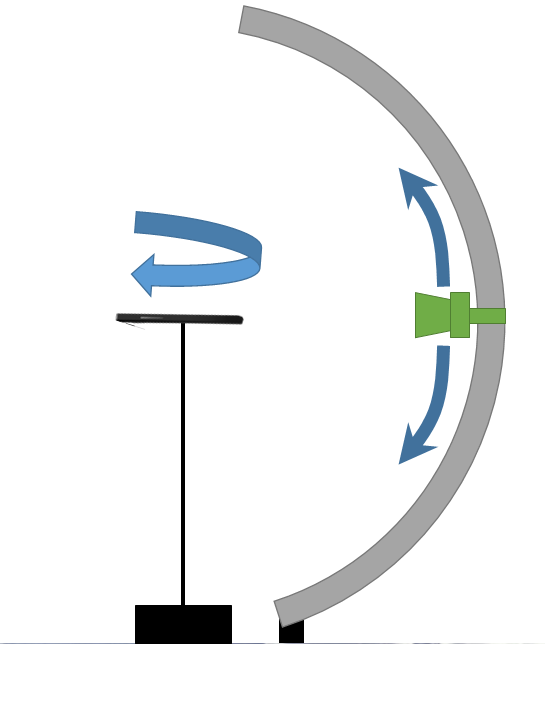
\includegraphics[height=8cm, width=8cm,keepaspectratio]{afbeeldingen/opstelling_pptx.png}
			    \caption{A sketch of the measurement set-up}
			    \label{fig:opstelling_pptx}
        \end{subfigure}%
        \quad %add desired spacing between images, e. g. ~, \quad, \qquad, \hfill etc.
          %(or a blank line to force the subfigure onto a new line)
        \begin{subfigure}[t]{0.5\textwidth}
                \centering
    			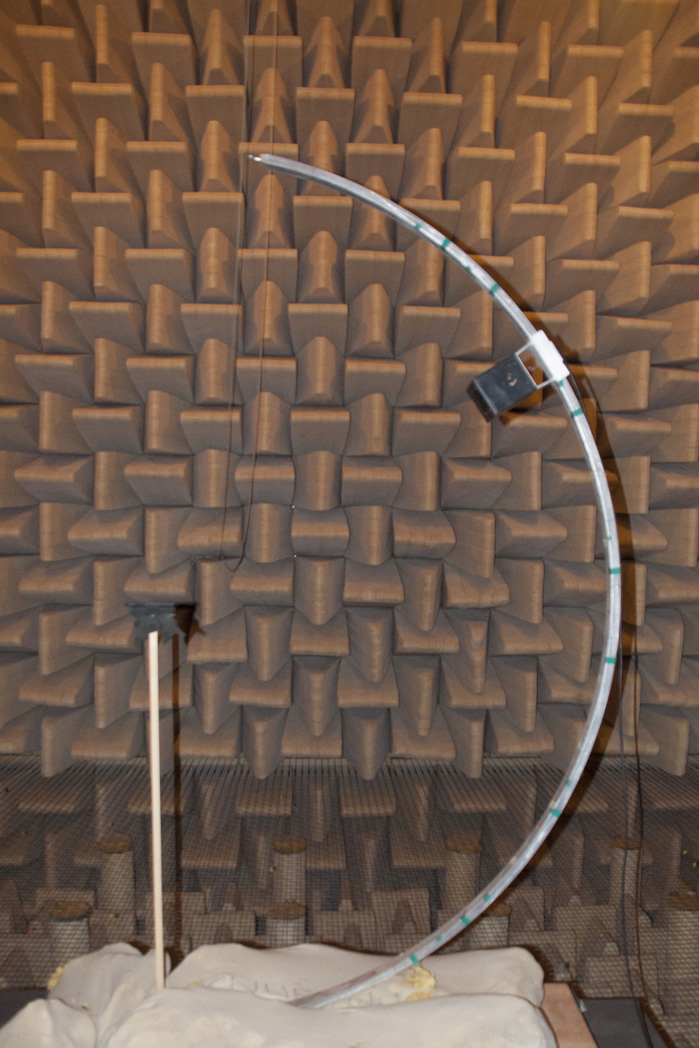
\includegraphics[height=8cm]{cover/onzecover.jpg}
			    \caption{A picture of the measurement set-up in the anechoic room at the Faculty of TNW at the Delft University of Technology}
			    \label{fig:opstelling_foto}
        \end{subfigure}
        \caption{Measurement set-up}
        \label{fig:opstelling_beide}
\end{figure}

In order to determine the directivity of the smartphone microphone, the impulse response of the microphone is measured in the anechoic room at the Delft University of Technology.
This room gives as little disturbance as possible from the surroundings.
Figure \ref{fig:opstelling_beide} shows the final measurement set-up, this set-up is already presented here to clarify the terms of the hardware.
As mentioned earlier, \nexus \cite{nexus5} is used and from now on the term $\it{smartphone}$ will refer to this specific phone. 

An aluminium arc with a radius of 1.21 meter will be positioned in the middle of the anechoic room.
This arc has a range from $-75^\circ$ tot $75^\circ$ (as a reference: $0^\circ$ is the horizon). A loudspeaker (with a length of 0.21 meter) is attached to this arc, which can be moved along the arc.
The loudspeaker and accompanying hanging system have a length of 0.21 meter, so the radius of the arc with loudspeaker is 1 meter. 

The phone is positioned on a turntable\footnote{This turntable is a part of the remote controllable Br\"uel \& Kj\ae r 9640 turntable system. \cite{manual:turntable}} in such a way that the distance between the speaker cone and the smartphone microphone is 1 meter for all measurements.
This turntable can only be turned in full degrees.

In order to record the sound on the smartphone, an application specifically made for this project was used, which allowed the smartphone to send the recordings via WiFi directly to \matlab.
The implementation of this smartphone application is detailed in \cite{BAP:RoySjoerd}.
The audio source consisted of a loudspeaker connected to a high-fidelity audio interface, an RME FireFace 800 \cite{manual:fireface}, connected to an audio amplifier\footnote{The amplifier that was used is a custom-built 8-channel amplifier built around the Philips TDA8560Q integrated circuit, capable of delivering 25W per channel into a 4$\Omega$ load.}.
The loudspeaker used, is a Tymphany 4" Midrange loudspeaker, type number M10MD-39-08 \cite{manual:loudspeaker}, which specifications can be found in Figure \ref{fig:app:hardware:loudspeaker}. 
This speaker is contained by a custom enclosure, for placement on the arc.

A Br\"uel \& Kj\ae r Free-field microphone \cite{manual:microphone} was available to use to determine the impulse response of the acoustic equipment without the disturbance by the smartphone microphone.
Specifications of this microphone can be found in Figure \ref{fig:app:hardware:mic}.

\section{Sampling scheme}
\label{sec:sampl_scheme}
There are many different ways to sample a sphere \cite{Zhang2012575}, as also discussed in Section \ref{sec:rel_res:sampl_sch}.
The turntable can be controlled with \matlab, the elevation of the loudspeaker on the arc however has to be adjusted by hand. Therefore, sampling schemes with as few manual operations as possible will be considered.
Replacing the loudspeaker is very time consuming and therefore undesirable.

To minimize the error margins, a maximum distance between two sampling points of half the minimum wavelength of the desired signal is taken into account.
A speed of sound of $v_\text{air}=344$ m/s is considered and the maximum frequency in a human voice is around $f_{\text{voice}_\text{max}}=8$ kHz \cite{hospital}, although for most applications in communication and speech enhancement a maximum of just 3.5 kHz is taken into account \cite[p.~58]{book:jorge_speechenhancement}.
Because the objective of this project concerns application in speech, frequencies above 8 kHz are of less value.
This gives a maximum distance between two sampling points of 2.15 cm \eqref{eqn:ontwerp_afstandmin}.

The sphere which will be sampled, is the sphere with centre the microphone of the smartphone and radius the length of the smartphone.
Within this sphere the behaviour of the sound is influenced by the smartphone and outside this sphere not, so the choice for the smallest sphere is made.
The smartphone has a length of $\ell_\text{phone}=13.87$ cm. The length of the equator of the sphere is $\ell_\text{eq}=2\pi\ell_\text{phone}\approx87.1$ cm.

There are two sampling schemes taken in account, which both feature a low number of movements about the $\phi$-direction, which shortens the execution time of the experiment,

\begin{equation}
\label{eqn:ontwerp_afstandmin}
\Delta\ell_\text{max}=\dfrac{\lambda_\text{min}}{2}=\dfrac{1}{2}\dfrac{v_\text{air}}{f_{\text{voice}_\text{max}}}=\dfrac{344}{16000}=2.15\text{ cm}.
\end{equation}

\subsection{Equiangular}
\label{ssec:equiangular}
An equiangular sampling scheme has equal angles between two neighbouring samples, so the sphere is divided into longitudes and latitudes.
In the direction of $\theta$ samples will be taken over $360^\circ$ and in the $\phi$-direction over $180^\circ$.
It is therefore important that the difference in angle between two sampling points is a common divisor of 180 and 360.
The distance around the equator is the circle with the largest distance between two sampling points on the sphere. 
On the equator the maximum distance between two sampling points thus is\footnote{For small angles the distance over the sphere is approximately the same as the direct distance, therefore this equation will be used.} 
\begin{equation*}
\Delta\ell_\text{max}\geq\ell_\text{eq}\cdot\dfrac{360^\circ}{\Delta\theta}.
\end{equation*}
The largest common divisor smaller than 8.9 is 7.5.
This yields 24 longitudes and 48 latitudes, for a total of $23\cdot 48+2=1106$ sampling points (when taken into account that on the poles there is only one sampling point).

In practice this cannot be done, because the turntable only turns in full degrees.
The first common divisor smaller than 8.9 is 6, this gives 30 longitudes and 60 latitudes, so a total of $29\cdot60+2=1742$ sampling points.
It would be more comprehensive to choose angles of $9^\circ$, which lowers the largest frequency, but it is more practical because it results in $19\cdot 40+2=762$ sampling points.

\subsection{IGLOO}
The other sampling scheme taken into account is the IGLOO sampling scheme \cite{Zhang2012575}.
The IGLOO sampling scheme divides the surface of the sphere in 12 faces, from now on called base faces, of approximately the same surface area.
The following base faces are used:
\begin{multicols}{2}
\begin{itemize}
\item[]\textbf{North pole}
\item $\phi\in[0^\circ,60^\circ]$, $\theta\in[0^\circ,120^\circ]$
\item $\phi\in[0^\circ,60^\circ]$, $\theta\in[120^\circ,240^\circ]$
\item $\phi\in[0^\circ,60^\circ]$, $\theta\in[240^\circ,360^\circ]$
\item[]\textbf{Middle}
\item $\phi\in[60^\circ,120^\circ]$, $\theta\in[0^\circ,60^\circ]$
\item $\phi\in[60^\circ,120^\circ]$, $\theta\in[60^\circ,120^\circ]$
\item $\phi\in[60^\circ,120^\circ]$, $\theta\in[120^\circ,180^\circ]$
\item $\phi\in[60^\circ,120^\circ]$, $\theta\in[180^\circ,240^\circ]$
\item $\phi\in[60^\circ,120^\circ]$, $\theta\in[240^\circ,300^\circ]$
\item $\phi\in[60^\circ,120^\circ]$, $\theta\in[300^\circ,360^\circ]$
\item[]\textbf{South pole}
\item $\phi\in[120^\circ,180^\circ]$, $\theta\in[0^\circ,120^\circ]$
\item $\phi\in[120^\circ,180^\circ]$, $\theta\in[120^\circ,240^\circ]$
\item $\phi\in[120^\circ,180^\circ]$, $\theta\in[240^\circ,360^\circ]$.
\end{itemize}
\end{multicols}
A sphere, partitioned in this way, with 64 sampling points per base face is shown in Figure \ref{fig:IGLOO}.

Assuming the same minimal distance between two sampling points on the equator of $\Delta\ell$, the sphere will be divided with $\Delta\phi=7.5^\circ$, because $\phi\in[0^\circ,180^\circ]$ can be divided in three parts of $60^\circ$.
$\Delta\theta_\text{middle}=7.5^\circ$ in the middle, because this can also be divided in pieces of $60^\circ$.
This gives a total number of sampling points in the middle part of $s_\text{middle}=7\cdot48=336$.

For the pole faces the sampling is not equiangular like in the middle part.
The following is applicable to both the north as the south pole of the sphere.
The $\Delta\phi=7.5$ is the same as in the middle part.
Assume $\Delta\theta_\text{pole}$ \eqref{eq:delta_pole} and $\Delta\theta$ have to be a common divisor of 120.
$\ell_{60^\circ}=2\cdot(\cos(30^\circ)\cdot\ell_\text{phone})\cdot\pi=74.98$ cm.
It then follows that $\Delta\theta_\text{pole}\leq10.32^\circ$, so a $\Delta\theta_\text{pole}=10^\circ$ will be used,

\begin{equation}
\label{eq:delta_pole}\Delta\theta_\text{pole}\leq\dfrac{360^\circ\cdot\Delta\ell_\text{max}}{\ell_{60^\circ}}.
\end{equation}

The poles are divided in three faces of $120^\circ$. The sampling points have to be placed so they still meet the requirement of $\Delta\ell_\text{max}=2.15$ cm.
Per face this gives a distribution like can be found in Figure \ref{fig:poolvlak}.
This ideal case is by coincidence also the sphere given in Figure \ref{fig:IGLOO} (page \pageref{fig:IGLOO}).

\begin{wrapfigure}{r}{0.5\textwidth}
    \centering
    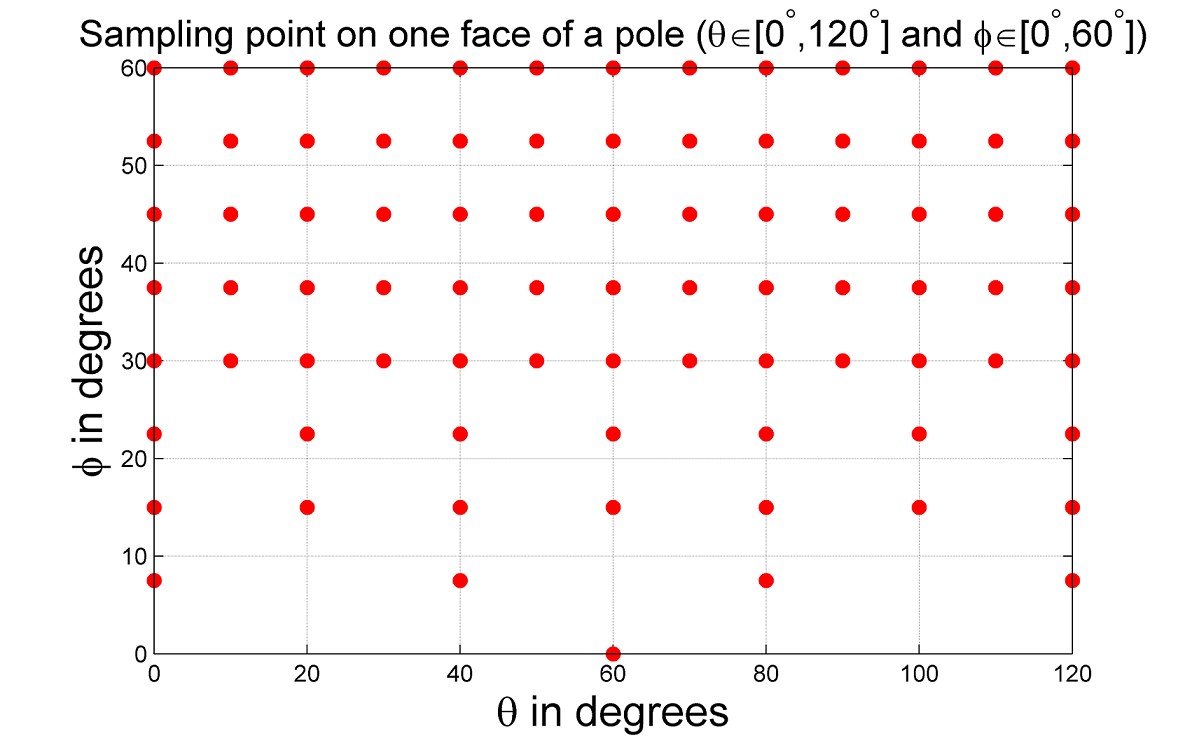
\includegraphics[width=0.5\textwidth]{afbeeldingen/poolvlak_optimaal.png}
    \caption{Distribution of sampling points on one face of the pole}
    \label{fig:poolvlak}
\end{wrapfigure}
This sampling scheme gives $s_\text{pole}=3\cdot(5\cdot12+2\cdot6+3)+1=226$ sampling points at the poles.
The full sampling scheme gives a total of 788 sampling points.
This theoretical case is not usable, because the turntable cannot turn half degrees. Because the middle of sphere has to be sampled equiangular, this gives $\Delta\theta_\text{middle}=\Delta\phi=6^\circ$ (9 is no divisor of 60), from which oversampling follows and this gives much more datapoints than the 762 of the equiangular method.

\subsection{Sampling scheme of choice}
The IGLOO sampling scheme seems appropriate for smaller angles (or larger spheres), because the requirements at $\Delta\theta$ of being a common divisor of 60 and 120 are easy applicable for those cases.
The sampling scheme used for the measurements is the equiangular scheme, because it has less sampling points than the IGLOO method and it is accurate for frequencies up to\footnote{If the assumption from the beginning of section \ref{sec:sampl_scheme} is followed.}
\begin{equation*}
f_\text{measure}=\dfrac{360\cdot v_\text{air}}{2\cdot\Delta\theta\cdot\ell_\text{eq}}=\dfrac{360\cdot344}{2\cdot9\cdot0.871}\approx7898\text{ Hz.}
\end{equation*} 

According to the method of Ajdler et al. \cite[eq.~(5)]{Ajdler2005III273}, the density of this sampling scheme should be accurate enough for frequencies up to 21.9 kHz \eqref{eq:ajdler}, which is higher than the maximum tone a human can hear (about 20 kHz).
\begin{equation}
\label{eq:ajdler}
\omega_t=\dfrac{cl_\theta}{0.137}=\dfrac{v_\text{sound}\cdot\Delta\theta}{0.137}=\dfrac{334\cdot 9}{0.137}\approx 21.9 \text{ kHz}
\end{equation}

\section{The measurement set-up}
The decisions concerning the measurement set-up are based on the hardware, theory and techniques mentioned above. The choice of measurement scheme is already explained in the above section.

In case of the impulse response measurement methods, both the TSP and MLS methods are used.
These measurement techniques should give the same impulse response result, which makes them suitable to verify the measurements while measuring.
If both techniques gave the same result, the measurement can be assumed to be succeeded. 

\subsection{Settings}
As much equipment was used for these measurements, values for many parameters had to be chosen.
First of all, the sound volume settings of the loudspeaker need to be in the desired range: loud enough for the phone to register, but not so loud it could saturate or force the speaker.
The volume settings are verified by looking at the signal amplitude measured by the smartphone. Many smartphones operate an automatic gain control: a controlled signal output despite variation of the input signal. This automatic gain control could give distortions in the measurement results. Keeping the signal amplitude measured by the smartphone between 10\% to 15\% of its maximum amplitude scale will prevent this. 

For the setting of the volume of the computer, it was important to not let the audio interface clip.
The software belonging to the Fireface clearly shows whether there is clipping or not. 
The clipping could be prevented by lowering the volume of the operating system (Windows in this case) or multiplying the \matlab-generated signal with a gain factor.
The final used settings were a volume of 5\% in Windows and a gain factor of -7 dB (power-dB) in \matlab.

Generating and analysing the TSP and MLS signals is done with \matlab~ code by Thomas \cite{Thomas2006}.
In order to use these codes, the order of the TSP and MLS, and the number of repetitions of each signal had to be chosen.
At the \matlab~ side, we chose for both the MLS and the TSP a sequence of order 15, with ten repetitions.
These sequences were played and recorded with a sampling frequency of 48 kHz.
This sampling frequency gives a Nyquist frequency of 24 kHz, which is more than enough for our application (remember $f_{\text{voice}_\text{max}}=8$ kHz).
The combination of the length of the signal and the sampling frequency made it possible to do approximately two measurements per minute, if multiplied by 762, a full sphere takes about 6 hours to measure.
When also the time to check and the manual movements of the speaker are taken into account, a full sphere takes about 8 hours (one work day) to measure.
So these choices give a achievable time schedule, with a good resolution and frequency range.

Measurements were conducted on different days, so the results of different days may differ due to analogue settings on the amplifier.
Therefore some showed preliminary results will not be alike. 
In the next chapter, our choice of equalizing the different measurements will be explained.

\subsection{Hardware placement}
The measurement set-up is shown in Figure \ref{fig:opstelling_pptx}.
In this set-up the following settings will be tested:
\begin{itemize}
\item The smartphone in mid-air\\
To measure the smartphone in mid-air, it will be positioned on a small supporting stick, covered with foam.
The foam is sound absorbing and smaller than the phone.
It supports the phone but does not change the path of the sound.
For measurements $\phi\geq90^\circ$ the phone will be placed upside down on the foam and will be turned the other way around.
This way, the foam and the stick will disturb the signal as little as possible and the measurement will be the same as when the speaker is set-up larger than $\phi=90^\circ$.
\item The smartphone on a surface\\
For the measurements on a surface there is another set-up available: a plywood plate with dimensions of $290\times240\times8$ mm placed on a stick.
The difference between the impulse response in mid-air and the impulse response on a surface is interesting because it will show whether the directivity of the phone in mid-air is representative of the behaviour on a surface.
The overall goal is to use the directivity in a system in which the phones will be positioned on a surface. If the results on a table are too different from those in mid air, the conclusion may be that there is too much difference between mid-air and table to use the mid-air measurements in the beamforming algorithm.

The smartphone has two configurations on a surface:
\begin{itemize}
\item Face up\\
With the back of the phone on the table.
\item Face down\\
With the screen of the phone on the table.
\end{itemize}
\end{itemize}

The last part of the measurement set-up concerns angles on the arc larger than $75^\circ$ and smaller than $-75^\circ$, because the arc does not reach that far.
To reach angles in $[75,90]$ and $[-90,-75]$ the turntable can be placed at an angle, to cover the last $15^\circ$. For instance: to measure at an angle of $82^\circ$, the speaker will be set at $75^\circ$ and the table will be tilted $7^\circ$.
This of course causes the smartphone to slide, so it will be secured with double-sided tape (1 mm thick).

For the smartphone in mid-air at angles smaller than $-75^\circ$ the described set-up with the double-sided tape will be used, but with the smartphone turned upside down. For the set-up with the smartphone on a surface, this cannot be applied, so there will be no measurements done at angles lower than $-45^\circ$, because an audio signal coming from angles smaller than $0^\circ$ will probably be attenuated very fast.

For the measurements with the table, the same sampling sphere will be used.

Pictures of the measurement set-up can be found in Figure \ref{fig:app:overview} in Appendix \ref{app:setupoverview}.

\section{Expectations}
\label{sec:ms-expectations}
\begin{wrapfigure}{r}{0.4\textwidth}
        \centering
		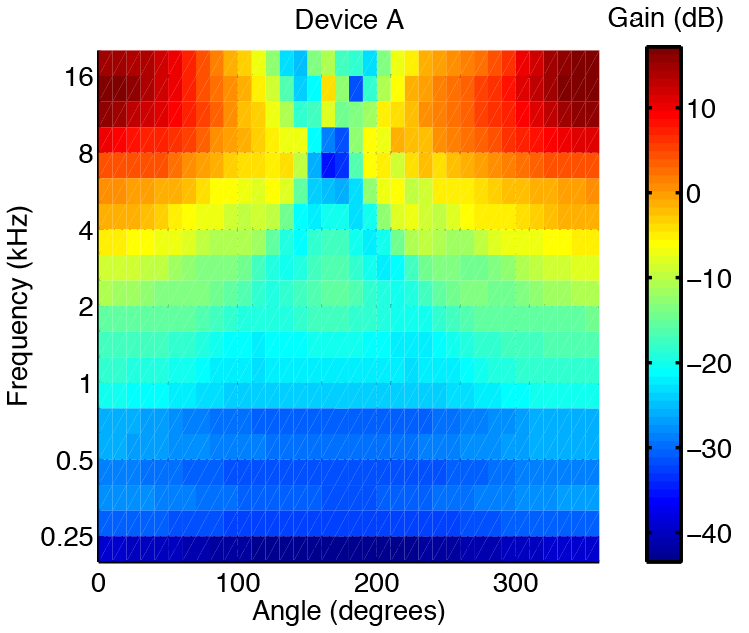
\includegraphics[]{afbeeldingen/device_a.png}
	    \caption[Device A from \cite{Gaubitch2014}]{Device A (\nexus) from Figure 1 from \cite{Gaubitch2014}: \textit{Average responses for three smartphone models in one-third octave bands. The results are presented as the average responses per smartphone model.}}
	    \label{fig:Gaubitch}
\end{wrapfigure}
There were already some expected results before the start of the measurements, mostly based on the measurements done previously by Gaubitch et al. \cite{Gaubitch2014} (Figure \ref{fig:Gaubitch}) and the physical characteristics of \nexus.
A non-symmetric directivity pattern in the $\theta$-axis is expected as the microphone of \nexus~ is not positioned in the middle of the smartphone but about two centimeters to the right. 
When turning the smartphone with the turntable, the microphone will thus not be completely turned away at $\theta=180^\circ$.
Furthermore, a turned away microphone should give less gain than a microphone directed towards the loudspeaker. 
Another expectation is that the measurements on a surface and in mid-air will give different results.
The surface is expected to cause reflections of the signal, so there will be multipath interference patterns to observe. For $\phi>90^\circ$ a high gain loss is expected because the surface will hamper the signal for such angles.  

\section{Preliminary results}
\label{sec:prelim_res}
The preliminary results of our measurements, plotted on a linear frequency axis, are shown in Figure \ref{fig:prelim:NX506_TSP_090_full} and \ref{fig:prelim:NX506_MLS_090_full} at the end of this chapter.
The first things to notice are the very low gains at the lowest and highest frequencies.
For the used decibel-scale 0 dB stands for no gain, which in this case means that the sent audiosignal is received with a gain of 1 at the microphone speaker.
The given decibel scale comes from the settings of the computer, equipment and the attenuation through the air, which all cause the signal to have very high weakening. 
These gains are the result of the loudspeaker, which frequency response for frequencies larger than 20 kHz is unknown \cite{manual:loudspeaker} and therefore considered low.
This can be seen in Figure \ref{fig:app:hardware:loudspeaker} in Appendix \ref{app:hardware-data}.
For frequencies smaller than approximately 125 Hz, the gain of the speaker is also decreasing very quickly.

To let not cloud our results by these limitations of the loudspeaker these plots are replotted with a limited frequency axis.
These are shown in Figure \ref{fig:prelim:NX506_TSP_090} and \ref{fig:prelim:NX506_MLS_090}.

One very important thing to notice is the presence of the line of lower gain at about 13.5 kHz.
This line was not expected, because these measurements were performed with the same smartphone as used by \cite{Gaubitch2014} (Figure \ref{fig:Gaubitch}).
Although these results are plotted in octave bands, there is no line of reduced gain visible around 13.5 kHz.
In the search for the cause, different smartphones, microphones and another loudspeaker of the same type \cite{manual:loudspeaker} were tested.
It is concluded that this reduced gain was probably a result of the use of the available banana connector cable of which 10 meter was used to transport the signal from the audio amplifier to the loudspeaker.
Because this cable is not as good as a normal transmission line (like a coaxial cable), there could be some frequency dependencies in the cable.

To determine the smartphone directivity, the frequency dependencies of the acoustic system need to be eliminated from the result.
Therefore the microphone \cite{manual:microphone} is used: the impulse response of the acoustic system is measured using both MLS and TSP and these measured responses are used for equalization.
How this equalization is done will be explained in Section \ref{sec:eq-design}.
The impulse responses given by the TSP and MLS signals are very much alike.
From now on all the plotted impulse responses will be those using the TSP-method as they are the same as the MLS results.

\section*{Measurements - Conclusion}
In this chapter an equiangular sampling scheme (with latitudes and longitudes $9^ \circ$ apart) for determining the smartphone directivity was presented.
Measurements using this scheme were conducted using the TSP and MLS impulse response determination techniques.
A summary of this chapter can be found in Appendix \ref{app:setupoverview}, for replication of our measurements.
The preliminary results of these measurements were given in Figure \ref{fig:prelim:NX506_090}. These results point out some effects, which did not match with the expectations. Therefore a way of equalizing the acquired dataset will be presented in the next chapter.

\begin{figure}[b!]
        \centering
        \begin{subfigure}[t]{0.5\textwidth}
                \centering
			    
    			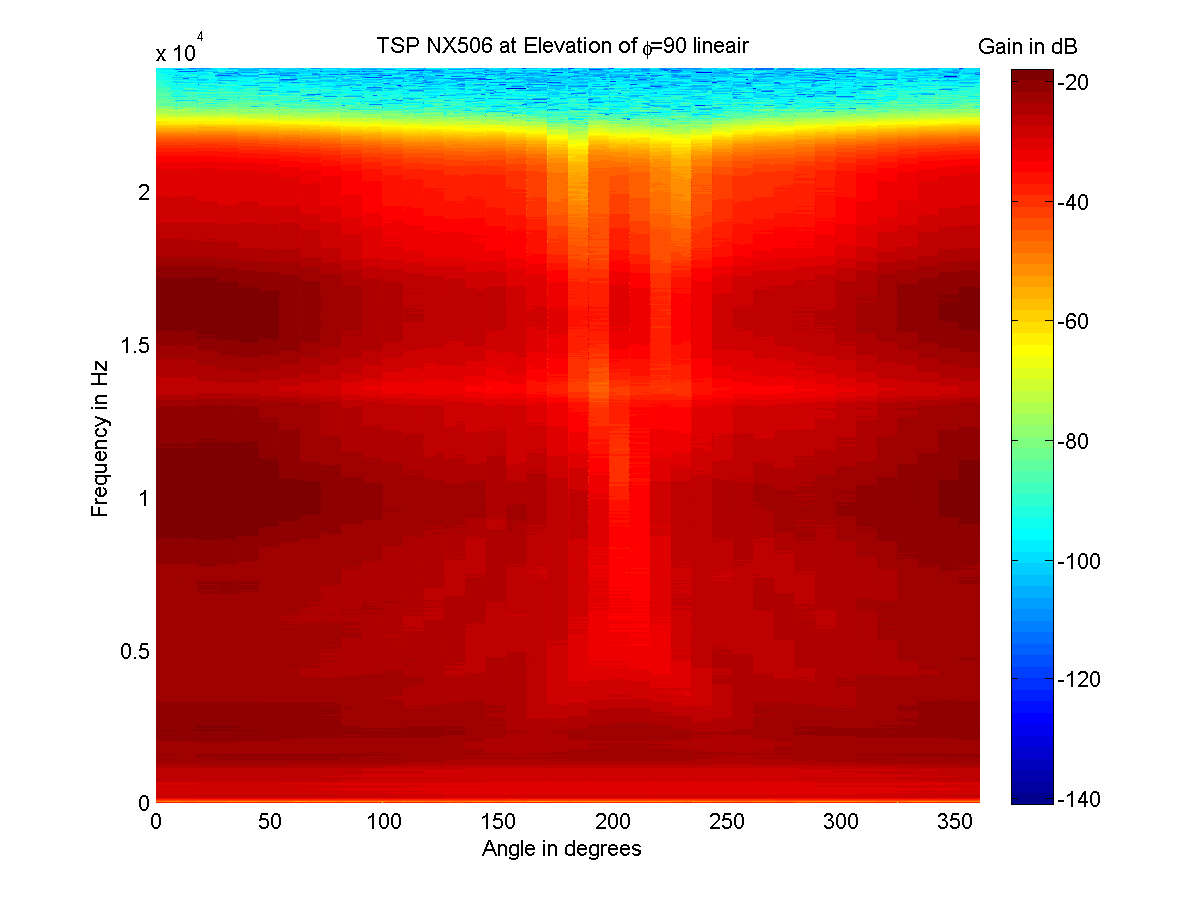
\includegraphics[width=\textwidth]{afbeeldingen/plots/NX506_TSP_090_lin_full.png}
    			\caption{TSP method}
			    \label{fig:prelim:NX506_TSP_090_full}
        \end{subfigure}~
        \begin{subfigure}[t]{0.5\textwidth}
                \centering
			    
    			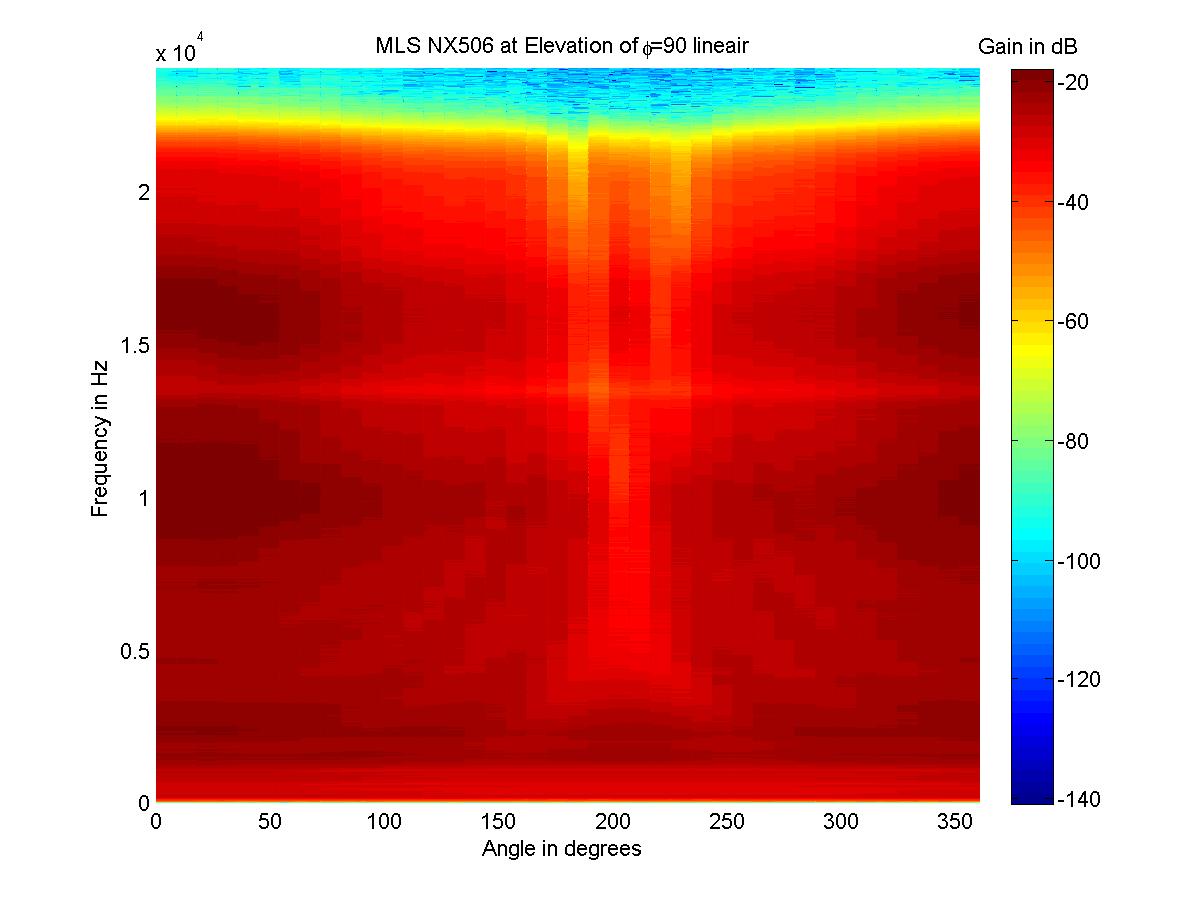
\includegraphics[width=\textwidth]{afbeeldingen/plots/NX506_MLS_090_lin_full.png}
    			\caption{MLS method}
			    \label{fig:prelim:NX506_MLS_090_full}
        \end{subfigure}

        \begin{subfigure}[t]{0.5\textwidth}
                \centering
			    
    			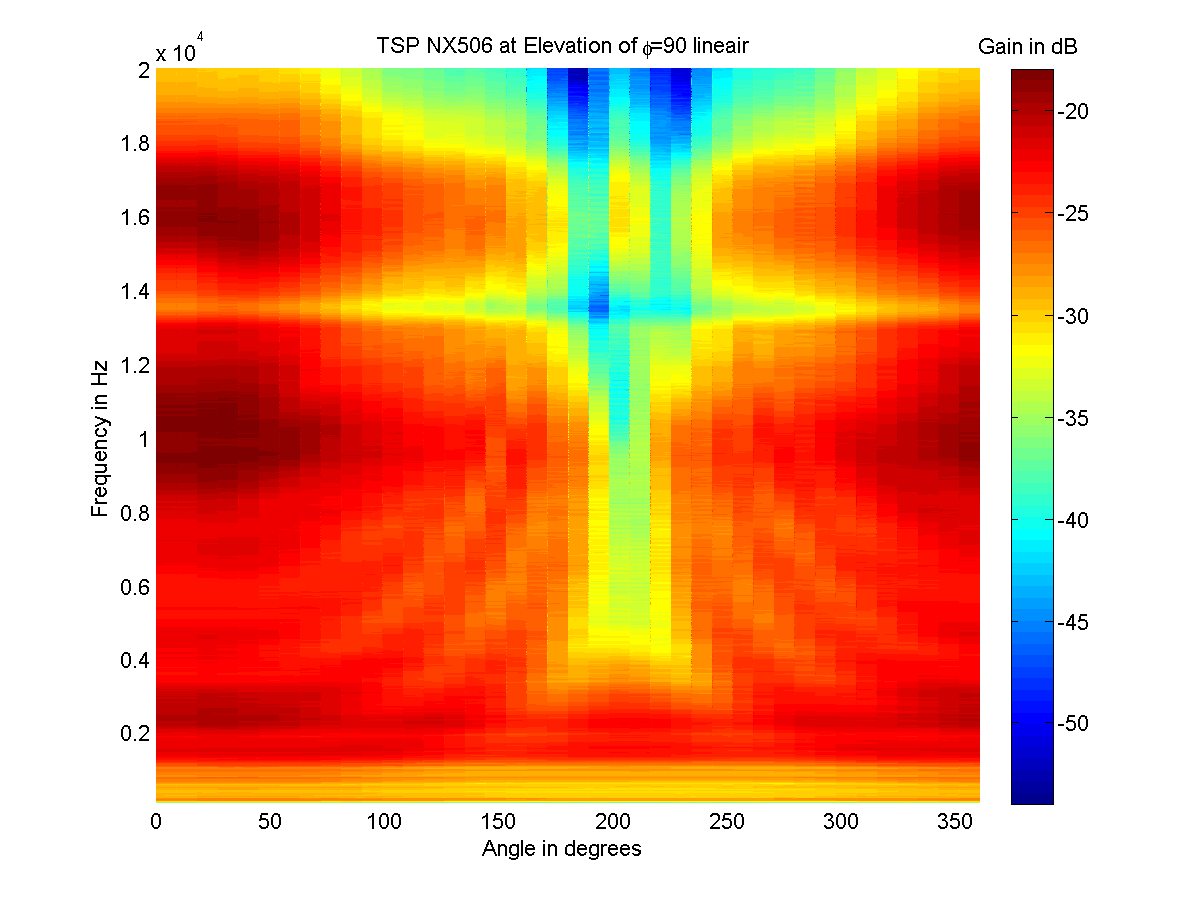
\includegraphics[width=\textwidth]{afbeeldingen/plots/NX506_TSP_090_lin.png}
    			\caption{TSP method, limited frequency axis}
			    \label{fig:prelim:NX506_TSP_090}
        \end{subfigure}~        
        \begin{subfigure}[t]{0.5\textwidth}
                \centering
			    
    			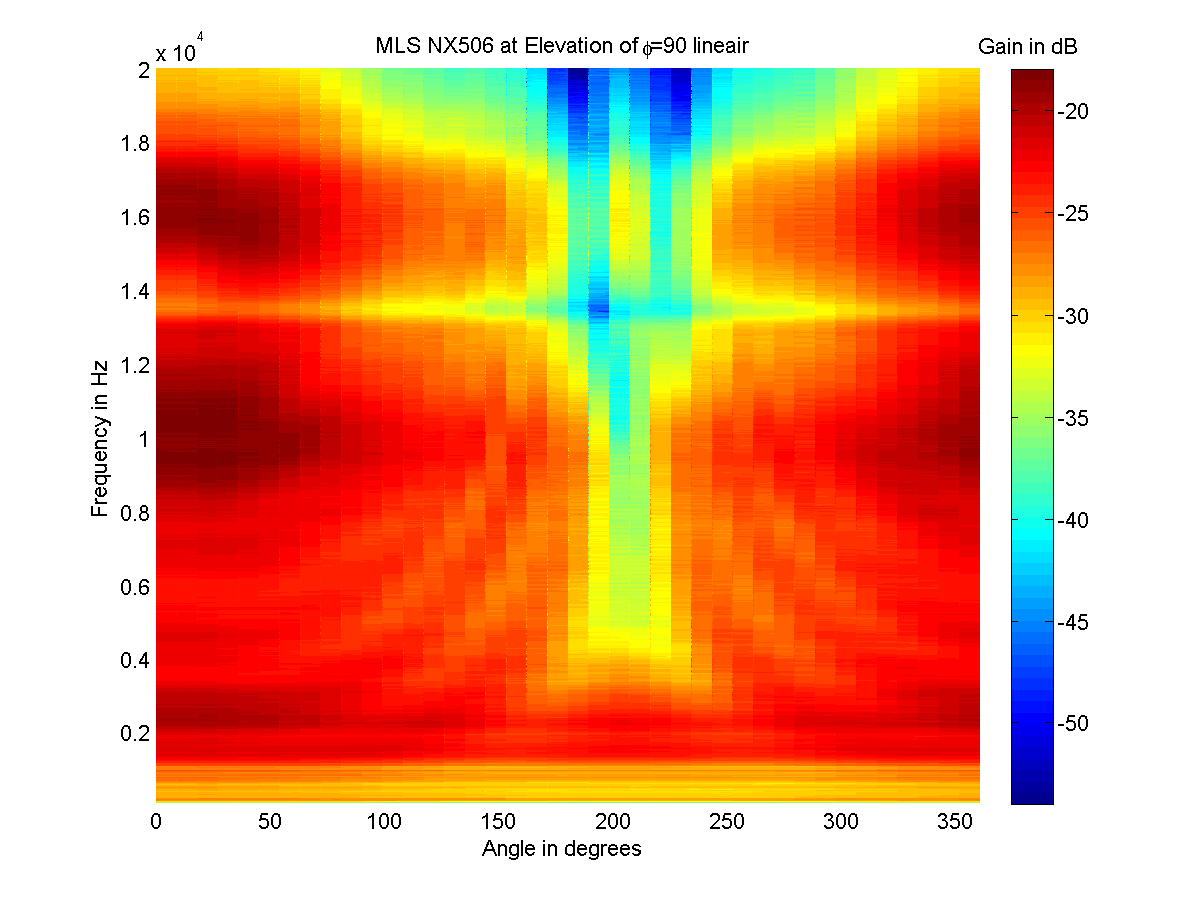
\includegraphics[width=\textwidth]{afbeeldingen/plots/NX506_MLS_090_lin.png}
    			\caption{MLS method, limited frequency axis}
			    \label{fig:prelim:NX506_MLS_090}
        \end{subfigure}
        
        \caption[Preliminary measurement results {\nexus} (6)]{Preliminary measurement results of {\nexus}, labelled with number 6, at $\phi=90$ degrees, with full frequency axis (from 0 Hz to 24 kHz) for the given methods.}
        \label{fig:prelim:NX506_090}
\end{figure}